\documentclass[11pt,a4paper]{article}

\usepackage[T1]{fontenc}
\usepackage[utf8]{inputenc}
\usepackage[brazil]{babel}
\usepackage{lmodern}
\usepackage[a4paper,margin=1.9cm]{geometry}
\usepackage{setspace}
\usepackage{booktabs}
\usepackage{array}
\usepackage{hyperref}
\usepackage{graphicx}
\usepackage{float}
\usepackage{placeins}
\usepackage{indentfirst}
\usepackage{enumitem}
\usepackage{longtable}

\setstretch{1.0}

\title{
Relatório Técnico de Ciência de Dados \\
Análise e Predição de Desfechos da Esquistossomose no Brasil
}

\author{
Luiz Gabriel Correia dos Santos (15639682) \\
Ana Paula de Abreu Batista (12688424) \\
Italo Carlos Martins Bresciani (15461782)
}

\date{\today}

\begin{document}

\maketitle

\section*{Resumo}

Este relatório apresenta uma análise exploratória, geoespacial e preditiva de casos de esquistossomose registrados no SINAN, utilizando extração automatizada via PySUS. Inicialmente, foi conduzida uma Análise Exploratória de Dados (EDA) para investigar a qualidade, estrutura e distribuição epidemiológica dos registros. Posteriormente, foram realizadas análises temporais e espaciais, com foco em padrões de incidência e concentração geográfica da doença. Por fim, aplicaram-se modelos supervisionados para predição de desfechos clínicos dos pacientes.

Os resultados evidenciaram forte concentração regional em Minas Gerais e Espírito Santo, além de limitações importantes da base relacionadas à ausência de variáveis clínicas densas e ao desbalanceamento entre classes. Entre os modelos avaliados, o XGBoost apresentou o melhor equilíbrio entre \textit{precision} e \textit{recall} para classes críticas como óbito e não cura, embora o desempenho ainda tenha sido limitado pela qualidade e estrutura dos dados disponíveis.

\section{Introdução}

A esquistossomose é uma doença parasitária crônica considerada um importante problema de saúde pública no Brasil, especialmente em regiões com infraestrutura sanitária precária e exposição frequente a coleções hídricas contaminadas.

O Sistema de Informação de Agravos de Notificação (SINAN) disponibiliza registros epidemiológicos em larga escala, permitindo investigações analíticas sobre distribuição espacial, dinâmica temporal e fatores associados aos desfechos clínicos da doença.

Neste trabalho, buscou-se responder à seguinte pergunta:

\begin{quote}
É possível, a partir do perfil epidemiológico e clínico de um caso notificado, construir um modelo capaz de predizer seu desfecho?
\end{quote}

Para isso, o projeto foi dividido em três grandes etapas:

\begin{enumerate}
    \item Análise Exploratória de Dados (EDA);
    \item Análise Geoespacial e Temporal;
    \item Aprendizado Supervisionado para predição de desfechos.
\end{enumerate}

\section{Base de Dados}

Os dados utilizados foram obtidos via biblioteca \texttt{PySUS}, utilizando registros do SINAN referentes ao agravo de esquistossomose (\texttt{ESQU}).

Após carregamento e concatenação das bases anuais, foram aplicados filtros de qualificação para construção da base analítica.

\subsection{Filtros Aplicados}

\begin{itemize}
    \item Casos positivos no exame Hoffman (\texttt{AN\_QUANT == 1});
    \item Remoção de desfechos ignorados;
    \item Exclusão de óbitos por causas não relacionadas à esquistossomose;
    \item Padronização de variáveis temporais e categóricas.
\end{itemize}

As classes finais utilizadas na modelagem foram:

\begin{itemize}
    \item 1 = Cura;
    \item 2 = Não Cura;
    \item 3 = Óbito por esquistossomose.
\end{itemize}

\section{Metodologia}

\subsection{Pré-processamento}

As seguintes etapas de tratamento foram realizadas:

\begin{itemize}
    \item Conversão de strings vazias para \texttt{NaN};
    \item Conversão de datas epidemiológicas;
    \item Padronização de códigos IBGE;
    \item Criação de variáveis derivadas temporais;
    \item Conversão de variáveis categóricas;
    \item Filtragem de inconsistências temporais.
\end{itemize}

\subsection{Análise Exploratória}

A EDA foi conduzida com os seguintes objetivos:

\begin{enumerate}
    \item Avaliar completude e consistência dos registros;
    \item Identificar padrões temporais;
    \item Analisar concentração geográfica;
    \item Caracterizar o perfil demográfico dos pacientes;
    \item Investigar padrões clínicos e terapêuticos.
\end{enumerate}

\subsection{Análise Geoespacial}

Foram realizadas análises espaciais focadas principalmente nos estados de Minas Gerais e Espírito Santo, identificados como áreas prioritárias devido à alta incidência média histórica.

A análise buscou identificar:

\begin{itemize}
    \item Municípios com maior concentração de casos;
    \item Relação entre distribuição espacial e hidrografia;
    \item Influência de fatores socioambientais;
    \item Possíveis focos locais de transmissão.
\end{itemize}

\subsection{Aprendizado Supervisionado}

O problema foi formulado como uma tarefa de classificação multiclasse supervisionada.

Os modelos baseline avaliados foram:

\begin{itemize}
    \item Regressão Logística;
    \item XGBoost;
    \item Versões com e sem PCA.
\end{itemize}

A estratégia de avaliação priorizou:

\begin{itemize}
    \item Recall para classes críticas;
    \item F1-macro;
    \item Precision;
    \item Comparação entre trade-offs clínicos.
\end{itemize}

\section{Resultados}

\subsection{Tendência Temporal}

Observou-se uma redução significativa no número de casos notificados entre 2007 e 2025, embora com oscilações relevantes em determinados períodos.

\begin{figure}[H]
\centering
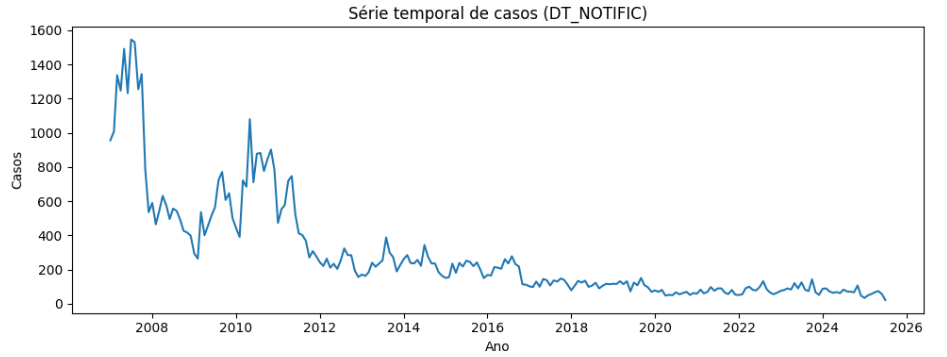
\includegraphics[width=\textwidth]{temporal.png}
\caption{Tendência temporal de casos de esquistossomose.}
\end{figure}

Os resultados sugerem avanços no controle da doença, possivelmente relacionados à ampliação do saneamento básico e melhorias em estratégias de vigilância epidemiológica.

\subsection{Distribuição Geográfica}

Minas Gerais e Espírito Santo apresentaram as maiores incidências médias por 100 mil habitantes no período analisado.

\begin{figure}[H]
\centering
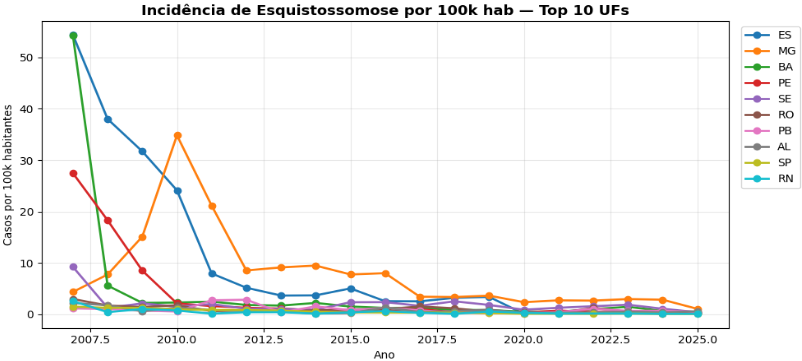
\includegraphics[width=\textwidth]{incidencia.png}
\caption{Incidência média por UF.}
\end{figure}

A concentração dos casos nesses estados motivou análises geoespaciais mais aprofundadas.

\subsection{Focos Municipais}

Foi realizada uma análise visual comparando a distribuição espacial dos municípios com maior concentração de casos e a presença da bacia do Rio São Francisco. Os resultados não indicaram relação espacial evidente entre os principais focos de notificação e a proximidade com a bacia hidrográfica principal da região.

Esse resultado sugere que a dinâmica de transmissão da esquistossomose pode estar mais associada a fatores locais do que à presença dos grandes cursos d'água. Entre os fatores potencialmente mais relevantes destacam-se:

\begin{itemize}
    \item saneamento básico precário;
    \item coleções hídricas menores e áreas de água parada;
    \item presença do hospedeiro intermediário;
    \item condições socioeconômicas locais.
\end{itemize}

Dessa forma, embora não tenha sido observada associação visual relevante com a bacia do Rio São Francisco, análises futuras podem incorporar outros corpos d'água regionais, como lagoas, açudes e pequenas coleções hídricas, buscando investigar com maior precisão possíveis influências ambientais na transmissão da doença.

\subsection{Tempo de Encerramento}

A análise do tempo de encerramento dos casos mostrou diferenças relevantes entre os desfechos clínicos.

\begin{itemize}
    \item Casos de óbito apresentaram mediana extremamente baixa;
    \item Casos de cura concentraram-se em torno de 10 dias;
    \item Casos de não cura exibiram distribuição bimodal.
\end{itemize}

A variável \texttt{tempo\_encerramento\_dias} demonstrou forte potencial discriminativo entre os desfechos analisados. Entretanto, essa variável deve ser interpretada com cautela em cenários preditivos, pois o encerramento do caso ocorre temporalmente muito próximo do registro do desfecho clínico, podendo introduzir vazamento de informação (\textit{data leakage}).

\subsection{Clusterização}

Foram realizadas tentativas exploratórias de clusterização com o objetivo de identificar possíveis agrupamentos naturais entre os casos notificados. Entretanto, os resultados não produziram agrupamentos clinicamente interpretáveis.

As principais limitações identificadas foram:

\begin{itemize}
    \item desbalanceamento entre features;
    \item alta cardinalidade de variáveis geográficas;
    \item ausência de informações clínicas detalhadas;
    \item forte dominância de atributos administrativos.
\end{itemize}

Dessa forma, concluiu-se que, para esta base específica, abordagens geoespaciais e modelos supervisionados apresentaram maior potencial analítico do que métodos não supervisionados.

\section{Predição de Desfecho Clínico}

\subsection{Features Utilizadas}

\begin{longtable}{p{5cm}p{6cm}p{3cm}}
\toprule
\textbf{Atributo} & \textbf{Descrição} & \textbf{Tipo} \\
\midrule
CS\_SEXO & Sexo do paciente & Categórico \\
CS\_GESTANT & Gestante & Categórico \\
CS\_RACA & Raça/cor & Categórico \\
CS\_ESCOL\_N & Escolaridade & Ordinal \\
FORMA & Forma clínica & Categórico \\
TRATAM & Tratamento realizado & Categórico \\
SG\_UF & UF de residência & Geográfico \\
COUFINF & UF provável de infecção & Geográfico \\
delay\_notificacao\_dias & Sintomas até notificação & Numérico \\
tempo\_encerramento\_dias & Sintomas até encerramento & Numérico \\
IDADE\_PROCESSADA & Idade do paciente & Numérico \\
\bottomrule
\end{longtable}

\subsection{Resultados dos Modelos}

\begin{figure}[H]
\centering
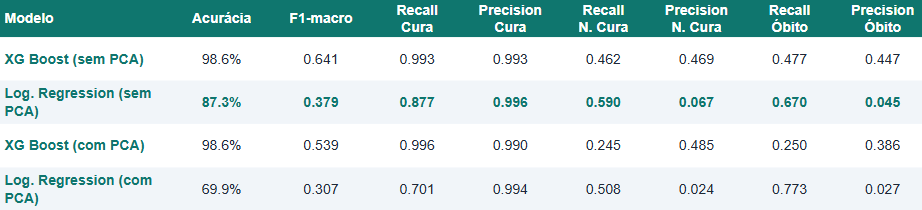
\includegraphics[width=\textwidth]{resultados.png}
\caption{Comparação entre modelos baseline}
\end{figure}

\subsection{Discussão dos Resultados}

Os principais achados foram:

\begin{itemize}
    \item O uso de PCA prejudicou o desempenho de ambos os modelos baseline, indicando perda de informação relevante durante a redução de dimensionalidade;

    \item O XGBoost apresentou o melhor equilíbrio entre \textit{precision} e \textit{recall} nas classes críticas (Não Cura e Óbito), alcançando aproximadamente 45--46\% tanto em cobertura quanto em acerto dessas classes;

    \item A regressão logística apresentou elevado número de falsos positivos, refletido em valores muito baixos de \textit{precision} para as classes minoritárias (entre 2\% e 7\%);

    \item A forte dominância da classe majoritária (Cura) influenciou significativamente as métricas globais, resultando em valores superiores a 99\% de \textit{precision} para essa classe em todos os modelos avaliados;

    \item O principal desafio permaneceu a identificação confiável de casos graves. Assim, o modelo ideal deve priorizar elevado \textit{recall} para classes críticas sem comprometer excessivamente a \textit{precision}.
\end{itemize}

\section{Limitações}

As principais limitações do projeto foram:

\begin{itemize}
    \item alta ausência de dados clínicos;
    \item inconsistências temporais;
    \item possível viés de subnotificação;
    \item alta cardinalidade de variáveis geográficas;
    \item desbalanceamento entre classes.
\end{itemize}

Além disso, variáveis potencialmente relevantes para prognóstico clínico não estavam disponíveis na base pública utilizada.

\section{Conclusão}

O projeto permitiu explorar diferentes abordagens analíticas aplicadas à epidemiologia computacional da esquistossomose.

Os resultados mostraram que:

\begin{itemize}
    \item Minas Gerais e Espírito Santo concentram áreas críticas de transmissão;
    
    \item fatores locais parecem exercer maior influência na dinâmica da doença do que grandes estruturas hidrográficas;
    
    \item análises geoespaciais forneceram insights epidemiológicos relevantes sobre concentração regional e possíveis focos locais de transmissão;
    
    \item modelos supervisionados apresentaram desempenho limitado, porém promissor, na identificação de desfechos graves;
    
    \item métricas globais elevadas foram fortemente influenciadas pelo desbalanceamento entre classes, não representando necessariamente elevada capacidade clínica preditiva;
    
    \item a qualidade e a disponibilidade limitada de variáveis clínicas restringiram o desempenho dos modelos desenvolvidos.
\end{itemize}

Como trabalhos futuros, recomenda-se que os próximos passos do projeto sigam os feedbacks obtidos ao longo da análise, visando aprimorar a robustez analítica e a capacidade preditiva dos modelos desenvolvidos:


\begin{enumerate}
    \item inclusão de variáveis ambientais e socioeconômicas externas, como indicadores de saneamento básico, vulnerabilidade social e cobertura de atenção básica;

    \item incorporação de dados geográficos relacionados à presença de lagoas, coleções hídricas e áreas de água parada, buscando caracterizar com maior precisão os ambientes favoráveis à transmissão da doença;

    \item aprofundamento da análise geoespacial utilizando Regionais de Saúde como principal unidade espacial de análise, por representarem melhor a dinâmica epidemiológica do que divisões administrativas convencionais;

    \item aplicação de métricas de autocorrelação espacial, como o Índice de Moran, para investigar padrões espaciais de concentração e dependência entre regiões;

    \item utilização de mapas de calor em escala logarítmica, permitindo melhor visualização de áreas com elevada discrepância no número de casos;

    \item realização de cortes temporais específicos para comparação entre diferentes períodos epidemiológicos e investigação de mudanças na dinâmica da doença ao longo do tempo;

    \item exploração de bases complementares, como dados do e-Gestor Atenção Básica, visando relacionar cobertura e infraestrutura de saúde pública com incidência e desfechos da esquistossomose;

    \item investigação mais aprofundada de possíveis alterações epidemiológicas observadas a partir de 2017, buscando identificar fatores associados às mudanças nos padrões registrados.
\end{enumerate}
\end{document}
```
